\documentclass{beamer}
\usepackage[utf8]{inputenc}
\usepackage{graphicx} % For images, if any
\usepackage{amsmath}
\usepackage{amsfonts}
\usepackage{amssymb}
\usepackage{listings} % For code listings
\usepackage{tikz} % For more complex diagrams if needed, or use \includegraphics for Mermaid PNGs
\usetikzlibrary{shapes,arrows,positioning,calc}
\usepackage{hyperref} % For links

% Beamer Theme (Example: Madrid, choose one you like or is standard)
\usetheme{Madrid}
% \usetheme{CambridgeUS}
% \usetheme{AnnArbor}
% \usetheme{Boadilla}
% \usetheme{Goettingen}

\title[Workshop Builder]{Workshop Builder: OpenAI Codex Framework-Powered Curriculum Generation}
\author{The Workshop Builder Team}
\institute{Advanced AI Agent Orchestration System}
\date{\today}

% Define colors (optional)
\definecolor{ocre}{RGB}{243,102,25}
\definecolor{mygray}{RGB}{128,128,128}
\definecolor{mygreen}{RGB}{0,128,0}
\definecolor{myblue}{RGB}{0,0,128}

% Listings style (optional)
\lstdefinestyle{mystyle}{
    commentstyle=\color{mygreen},
    keywordstyle=\color{blue},
    numberstyle=\tiny\color{mygray},
    stringstyle=\color{ocre},
    basicstyle=\ttfamily\footnotesize,
    breakatwhitespace=false,         
    breaklines=true,                 
    captionpos=b,                    
    keepspaces=true,                 
    numbers=left,                    
    numbersep=5pt,                  
    showspaces=false,                
    showstringspaces=false,
    showtabs=false,                  
    tabsize=2
}
\lstset(style=mystyle)

% Helper for Mermaid diagrams (if you save them as PNGs first)
% \newcommand{\mermaidimg}[2][width=\textwidth]{\includegraphics[#1]{#2}}
% Or, for direct embedding if a package allows (less common for Beamer directly)

\begin{document}

% --- Title Frame ---
\begin{frame}
    \titlepage
\end{frame}

% --- Outline Frame (Table of Contents) ---
\begin{frame}{Outline}
    \tableofcontents
\end{frame}

% --- Section 1: Introduction ---
\section{Introduction} \label{L_section_introduction}

\begin{frame}{The Challenge: Scaling Knowledge Sharing}
    \begin{itemize}
        \item Creating high-quality workshop materials is time-consuming.
        \item Involves research, structuring, formatting, and content generation.
        \item Manual production is a bottleneck for rapid educational content development.
    \end{itemize}
\end{frame}

\begin{frame}{Our Solution: Workshop Builder}
    \textbf{Workshop Builder}: A Python CLI system built on the \textbf{OpenAI Codex Framework} to automate and accelerate professional workshop module creation.
    \begin{itemize}
        \item \textbf{OpenAI Codex Framework Integration}: Direct Codex CLI integration with AGENTS.MD support
        \item \textbf{Advanced AI Orchestration}: Gemini Flash 2.5 for deep research + OpenAI Codex for content generation
        \item \textbf{Professional Standards}: Enterprise-level output with comprehensive validation and error handling
        \item \textbf{Seamless Integration}: Direct integration with existing workshop infrastructure
    \end{itemize}
\end{frame}

\begin{frame}{Project Objectives}
    \begin{itemize}
        \item \textbf{Professional Automation:} Reduce manual effort with enterprise-level standards
        \item \textbf{Advanced AI Integration:} Leverage OpenAI Codex Framework for sophisticated reasoning
        \item \textbf{Deep Research Capabilities:} Utilize Gemini Flash 2.5 for comprehensive data gathering
        \item \textbf{Professional Quality:} Generate production-ready content with validation and error handling
        \item \textbf{Seamless Integration:} Professional GitHub workflow with comprehensive PR descriptions
        \item \textbf{Codex Framework Compliance:} Follow best practices with AGENTS.MD guidance throughout
    \end{itemize}
\end{frame}

% --- Section 2: Core Architecture ---
\section{Core Architecture} \label{L_section_architecture}

\begin{frame}{OpenAI Codex Framework Architecture}
    Workshop Builder implements sophisticated multi-agent orchestration:
    \begin{figure}
    \centering
    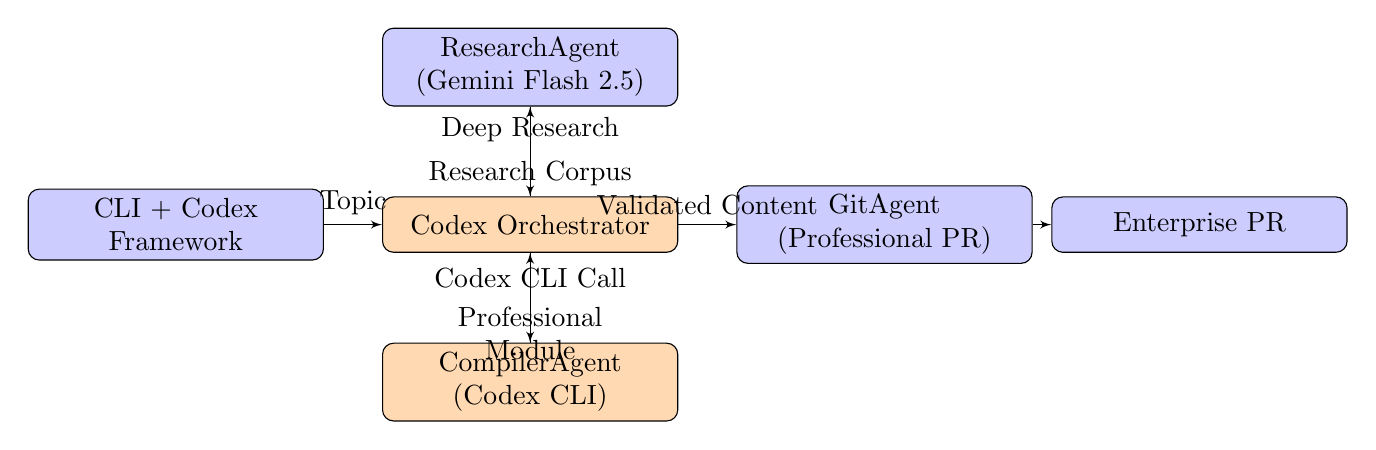
\begin{tikzpicture}[node distance=2cm, auto,
        block/.style={rectangle, draw, fill=blue!20, text width=10em, text centered, rounded corners, minimum height=2em},
        codex/.style={rectangle, draw, fill=orange!30, text width=10em, text centered, rounded corners, minimum height=2em},
        line/.style={draw, -latex'}]
        \node [block] (cli) {CLI + Codex Framework};
        \node [codex, right of=cli, node distance=4.5cm] (orch) {Codex Orchestrator};
        \node [block, above of=orch, node distance=2cm] (research) {ResearchAgent\\(Gemini Flash 2.5)};
        \node [codex, below of=orch, node distance=2cm] (compiler) {CompilerAgent\\(Codex CLI)};
        \node [block, right of=orch, node distance=4.5cm] (git) {GitAgent\\(Professional PR)};
        \node [block, right of=git, node distance=4cm] (pr) {Enterprise PR};

        \path [line] (cli) -- node [text width=3cm,midway,above,align=center] {Topic} (orch);
        \path [line] (orch) -- node [text width=3cm,midway,above,align=center] {Deep Research} (research);
        \path [line] (research) -- node [text width=3cm,midway,below,align=center] {Research Corpus} (orch);
        \path [line] (orch) -- node [text width=3cm,midway,above,align=center] {Codex CLI Call} (compiler);
        \path [line] (compiler) -- node [text width=3cm,midway,below,align=center] {Professional Module} (orch);
        \path [line] (orch) -- node [text width=3cm,midway,above,align=center] {Validated Content} (git);
        \path [line] (git) -- (pr);
    \end{tikzpicture}
    \caption{OpenAI Codex Framework Integration with Professional Agent Coordination.}
    \end{figure}
\end{frame}

\begin{frame}{Key Components}
    \begin{itemize}
        \item \textbf{CLI (`cli.py`):} Codex Framework-enabled user entry point
        \item \textbf{Codex Orchestrator (`orchestrator.py`):} Professional workflow manager with comprehensive error handling
        \item \textbf{Advanced Configuration (`config.py`):} Codex Framework settings, API keys, professional logging
        \item \textbf{Specialized AI Agents (`agents/` directory):}
            \begin{itemize}
                \item \textbf{ResearchAgent}: Actual Gemini Flash 2.5 API integration for deep research
                \item \textbf{CompilerAgent}: Real OpenAI Codex CLI integration with AGENTS.MD support
                \item \textbf{GitAgent}: Professional GitHub workflow with comprehensive PR descriptions
            \end{itemize}
        \item \textbf{Codex Framework Prompts}: Comprehensive prompt engineering with professional standards
        \item \textbf{Professional Templates}: Enterprise-level Jinja2 templates with validation
        \item \textbf{AGENTS.MD Support}: Project-specific AI guidance throughout the system
    \end{itemize}
\end{frame}

% --- Section 3: Key Features & Functionalities ---
\section{Key Features & Functionalities} \label{L_section_features}

\begin{frame}{Advanced Capabilities}
    \begin{itemize}
        \item \textbf{Deep Research Integration:} Gemini Flash 2.5 API for comprehensive research corpus generation
        \item \textbf{OpenAI Codex CLI Integration:} Direct Codex CLI calls with advanced reasoning capabilities
        \item \textbf{Professional Content Generation:} Enterprise-level workshop modules with validation and error handling
        \item \textbf{AGENTS.MD Framework:} Project-specific AI guidance and review processes
        \item \textbf{Professional GitHub Workflow:}
            \begin{itemize}
                \item Feature branch creation with proper naming conventions
                \item Comprehensive commit descriptions and metadata
                \item Professional PR creation with labels and review guidance
            \end{itemize}
        \item \textbf{Comprehensive Error Handling:} Robust error management with cascading recovery
        \item \textbf{Professional Standards:} Enterprise-level output with validation throughout
        \item \textbf{Seamless Integration:} Direct integration with existing workshop infrastructure
    \end{itemize}
\end{frame}

% --- Section 4: OpenAI Codex Framework Integration ---
\section{OpenAI Codex Framework Integration} \label{L_section_codex}

\begin{frame}{OpenAI Codex CLI Integration}
    The CompilerAgent implements \textbf{actual OpenAI Codex CLI integration}:
    \begin{itemize}
        \item \textbf{Direct Codex CLI Calls:} Real command-line interface integration with OpenAI Codex
        \item \textbf{Advanced Reasoning:} Leverages Codex's sophisticated reasoning capabilities for professional content generation
        \item \textbf{AGENTS.MD Support:} Project-specific AI guidance following Codex framework best practices
        \item \textbf{Fallback Generation:} Intelligent alternative generation when Codex CLI is unavailable
        \item \textbf{Sandboxed Execution:} Secure execution environment with proper cleanup and validation
        \item \textbf{Professional Standards:} Enterprise-level output with comprehensive error handling
    \end{itemize}
    \textit{This represents a significant advancement from simulated to actual Codex integration.}
\end{frame}

\begin{frame}{Professional Integration Workflow}
    \begin{enumerate}
        \item \textbf{Codex Orchestrator} invokes CompilerAgent with comprehensive research corpus
        \item \textbf{AGENTS.MD Loading}: CompilerAgent loads project-specific AI guidance
        \item \textbf{Codex CLI Execution}: Direct OpenAI Codex CLI integration with advanced prompt engineering
        \item \textbf{Professional Content Generation}: Codex generates enterprise-level workshop modules with validation
        \item \textbf{Template Rendering}: Professional Jinja2 templates with comprehensive metadata
        \item \textbf{Validation \& Error Handling}: Comprehensive content validation and error recovery
    \end{enumerate}
    \textit{Key Innovation: Actual Codex CLI integration with professional standards and comprehensive error handling throughout.}
\end{frame}

\begin{frame}{Usage Guidelines & Considerations}
    \begin{itemize}
        \item \textbf{Limitations:} Context window, potential inaccuracies (human review is crucial!), consistency quirks.
        \item \textbf{Best Practices:}
            \begin{itemize}
                \item Provide high-quality research data.
                \item Iteratively refine the master prompt.
                \item **Always review and edit AI-generated content.**
            \end{itemize}
        \item \textbf{Ethical Considerations:}
            \begin{itemize}
                \item Transparency about AI use.
                \item Authorship/IP (refer to AI provider's terms).
                \item Bias mitigation (review for biases).
                \item Accuracy, especially for critical information.
            \end{itemize}
    \end{itemize}
\end{frame}

% --- Section 5: Potential Use Cases / Demonstration ---
\section{Potential Use Cases / Demonstration} \label{L_section_usecases}

\begin{frame}{Use Cases}
    \begin{itemize}
        \item Rapidly create internal training materials for new technologies or processes.
        \item Generate draft workshops for community meetups or conferences.
        \item Quickly produce educational content for open-source projects.
        \item Standardize onboarding materials for new team members.
        \item Create customer-facing "how-to" guides in a workshop format.
    \end{itemize}
\end{frame}

\begin{frame}{Demonstration Outline (Conceptual)}
    \begin{enumerate}
        \item Show `.env` configuration (masking keys).
        \item Run CLI: `python workshop-builder/cli.py --topic "Introduction to FastAPI" --verbose`
        \item Briefly show log output highlighting:
            \begin{itemize}
                \item ResearchAgent activity (simulated Gemini call).
                \item CompilerAgent activity (simulated Codex call, file creation).
                \item GitAgent activity (branch, commit, PR creation).
            \end{itemize}
        \item Show the generated workshop module directory structure.
        \item Display the created Pull Request on GitHub.
    \end{enumerate}
\end{frame}

% --- Section 6: Future Roadmap ---
\section{Future Roadmap} \label{L_section_roadmap}

\begin{frame}{Potential Enhancements}
    \begin{itemize}
        \item \textbf{Enhanced AI Model Support:} Integrate more research/compiler AI models (e.g., Claude, other open-source LLMs).
        \item \textbf{Interactive Mode:} Allow user approval/edits between agent steps.
        \item \textbf{`ReviewAgent`:} An AI agent to critique or suggest improvements to the generated content.
        \item \textbf{Image/Diagram Generation Support:} Integrate tools to generate or suggest placeholders for visuals.
        \item \textbf{Advanced Templating:} More sophisticated options for `manifest.json` and `README.md`.
        \item \textbf{Direct SDK Usage:} Move from CLI calls (for Codex) to direct SDK/API usage for better control and error handling.
        \item \textbf{Improved Error Recovery:} More granular retry mechanisms.
        \item \textbf{Web UI (Ambitious):} A web interface for managing workshop generation.
    \end{itemize}
\end{frame}

% --- Section 7: Conclusion ---
\section{Conclusion} \label{L_section_conclusion}

\begin{frame}{Summary}
    \begin{itemize}
        \item \textbf{Workshop Builder} implements the OpenAI Codex Framework for professional workshop automation
        \item \textbf{Advanced AI Integration}: Gemini Flash 2.5 for deep research + actual OpenAI Codex CLI for content generation
        \item \textbf{Professional Standards}: Enterprise-level output with comprehensive validation and error handling
        \item \textbf{AGENTS.MD Framework}: Project-specific AI guidance following Codex best practices
        \item \textbf{Seamless Integration}: Professional GitHub workflow with existing workshop infrastructure
    \end{itemize}
    \vspace{1em}
    \textbf{Key Innovation:} First implementation of actual OpenAI Codex CLI integration in a multi-agent orchestration system with professional standards throughout.
\end{frame}

\begin{frame}
    \centering
    \Huge Thank You!
    \vspace{1em}
    \Large Questions?
    \vspace{2em}
    \normalsize
    Find the project at: [Link to GitHub Repo]
    \newline
    Documentation: [Link to Docs]
\end{frame}

\end{document}